\section{Results}\label{sec:results}

All experiments use the instances of Table~\ref{tab:instances} and the regime $\rho_s$ of Section~\ref{sec:data} unless stated otherwise. For each state and party we compute a certified bracket $[r_q,u_q)$ for every $\sigma^*(q)$: $r_q$ is the $q$-th robust margin of an independently verified plan, and $\sigma^*(q)<u_q$ is proved by an infeasibility certificate at a grid margin $u_q$ (grid step 0.5 points of two-party share; Section~\ref{sec:frontier}). Margins are reported as district two-party share $=50\%+m$. Lower bounds come from a county-aware recombination hill climber followed by exact large-neighbourhood search (Algorithm~\ref{alg:cegar} on restricted instances), and every improvement is then attacked by the certifying loop.

\subsection{Certified seat--safety frontiers}\label{sec:main}

Table~\ref{tab:capacity} states, for every state and party, the number of districts that can simultaneously reach 50\%, 55\% and 60\% of the two-party vote; a single number is an exact value of $F_\rho(m)$ (certified lower and upper bounds coincide) and an interval $a$--$b$ gives $a\le F_\rho(m)\le b$. Figure~\ref{fig:frontier2} shows the certified frontiers of the six two-district states with the region between the certified lower and upper staircases shaded (invisible when the bracket is a fraction of a point wide), Figure~\ref{fig:frontier3} those of the states with $3\le k\le5$, and Table~\ref{tab:spectrum} in the appendix lists every bracket for $\sigma^*(q)$.

\begin{table}[!tbp]
\centering\small
\caption{Certified seat--safety capacity at $\rho_s$ ($\pm1\%$, $k-1$ county splits, 2020 presidential two-party vote): number of districts that can simultaneously have at least the stated party share. Single number = exact; $a$--$b$ = certified interval.}\label{tab:capacity}
\adjustbox{max width=\linewidth}{\begin{tabular}{llrcccc}
\toprule
State & Party & $k$ & stat.\ share & $\ge50\%$ & $\ge55\%$ & $\ge60\%$ \\
\midrule
New Hampshire & D & 2 & 53.7\% & 2 & 1 & 0 \\
New Hampshire & R & 2 & 46.3\% & 0 & 0 & 0 \\
Maine & D & 2 & 54.7\% & 2 & 1 & 1 \\
Maine & R & 2 & 45.3\% & 1 & 0 & 0 \\
Rhode Island & D & 2 & 60.6\% & 2 & 2 & 2 \\
Rhode Island & R & 2 & 39.4\% & 0 & 0 & 0 \\
Idaho & D & 2 & 34.1\% & 0 & 0 & 0 \\
Idaho & R & 2 & 65.9\% & 2 & 2 & 2 \\
Montana & D & 2 & 41.6\% & 1 & 0 & 0 \\
Montana & R & 2 & 58.4\% & 2 & 2 & 1 \\
West Virginia & D & 2 & 30.2\% & 0 & 0 & 0 \\
West Virginia & R & 2 & 69.8\% & 2 & 2 & 2 \\
Nebraska & D & 3 & 40.2\% & 1--2 & 1 & 0--1 \\
Nebraska & R & 3 & 59.8\% & 3 & 3 & 2 \\
New Mexico & D & 3 & 55.5\% & 3 & 3 & 2 \\
New Mexico & R & 3 & 44.5\% & 2 & 1 & 1 \\
Arkansas & D & 4 & 35.8\% & 1--2 & 1 & 0--1 \\
Arkansas & R & 4 & 64.2\% & 4 & 4 & 4 \\
Iowa & D & 4 & 45.8\% & 3 & 2 & 1 \\
Iowa & R & 4 & 54.2\% & 4 & 3 & 2--3 \\
Kansas & D & 4 & 42.5\% & 2--3 & 1--2 & 1 \\
Kansas & R & 4 & 57.5\% & 4 & 3--4 & 3 \\
Mississippi & D & 4 & 41.6\% & 2--3 & 1--2 & 1--2 \\
Mississippi & R & 4 & 58.4\% & 4 & 4 & 3 \\
Nevada & D & 4 & 51.2\% & 3--4 & 2 & 2 \\
Nevada & R & 4 & 48.8\% & 3 & 2 & 0--1 \\
Utah & D & 4 & 39.3\% & 2 & 1 & 1 \\
Utah & R & 4 & 60.7\% & 4 & 4 & 3--4 \\
Connecticut & D & 5 & 60.2\% & 5 & 5 & 5 \\
Connecticut & R & 5 & 39.8\% & 1 & 0 & 0 \\
Oklahoma & D & 5 & 33.1\% & 1--2 & 0--1 & 0--1 \\
Oklahoma & R & 5 & 66.9\% & 5 & 5 & 5 \\
\bottomrule
\end{tabular}
}
\end{table}

\begin{figure}[!tbp]
\centering
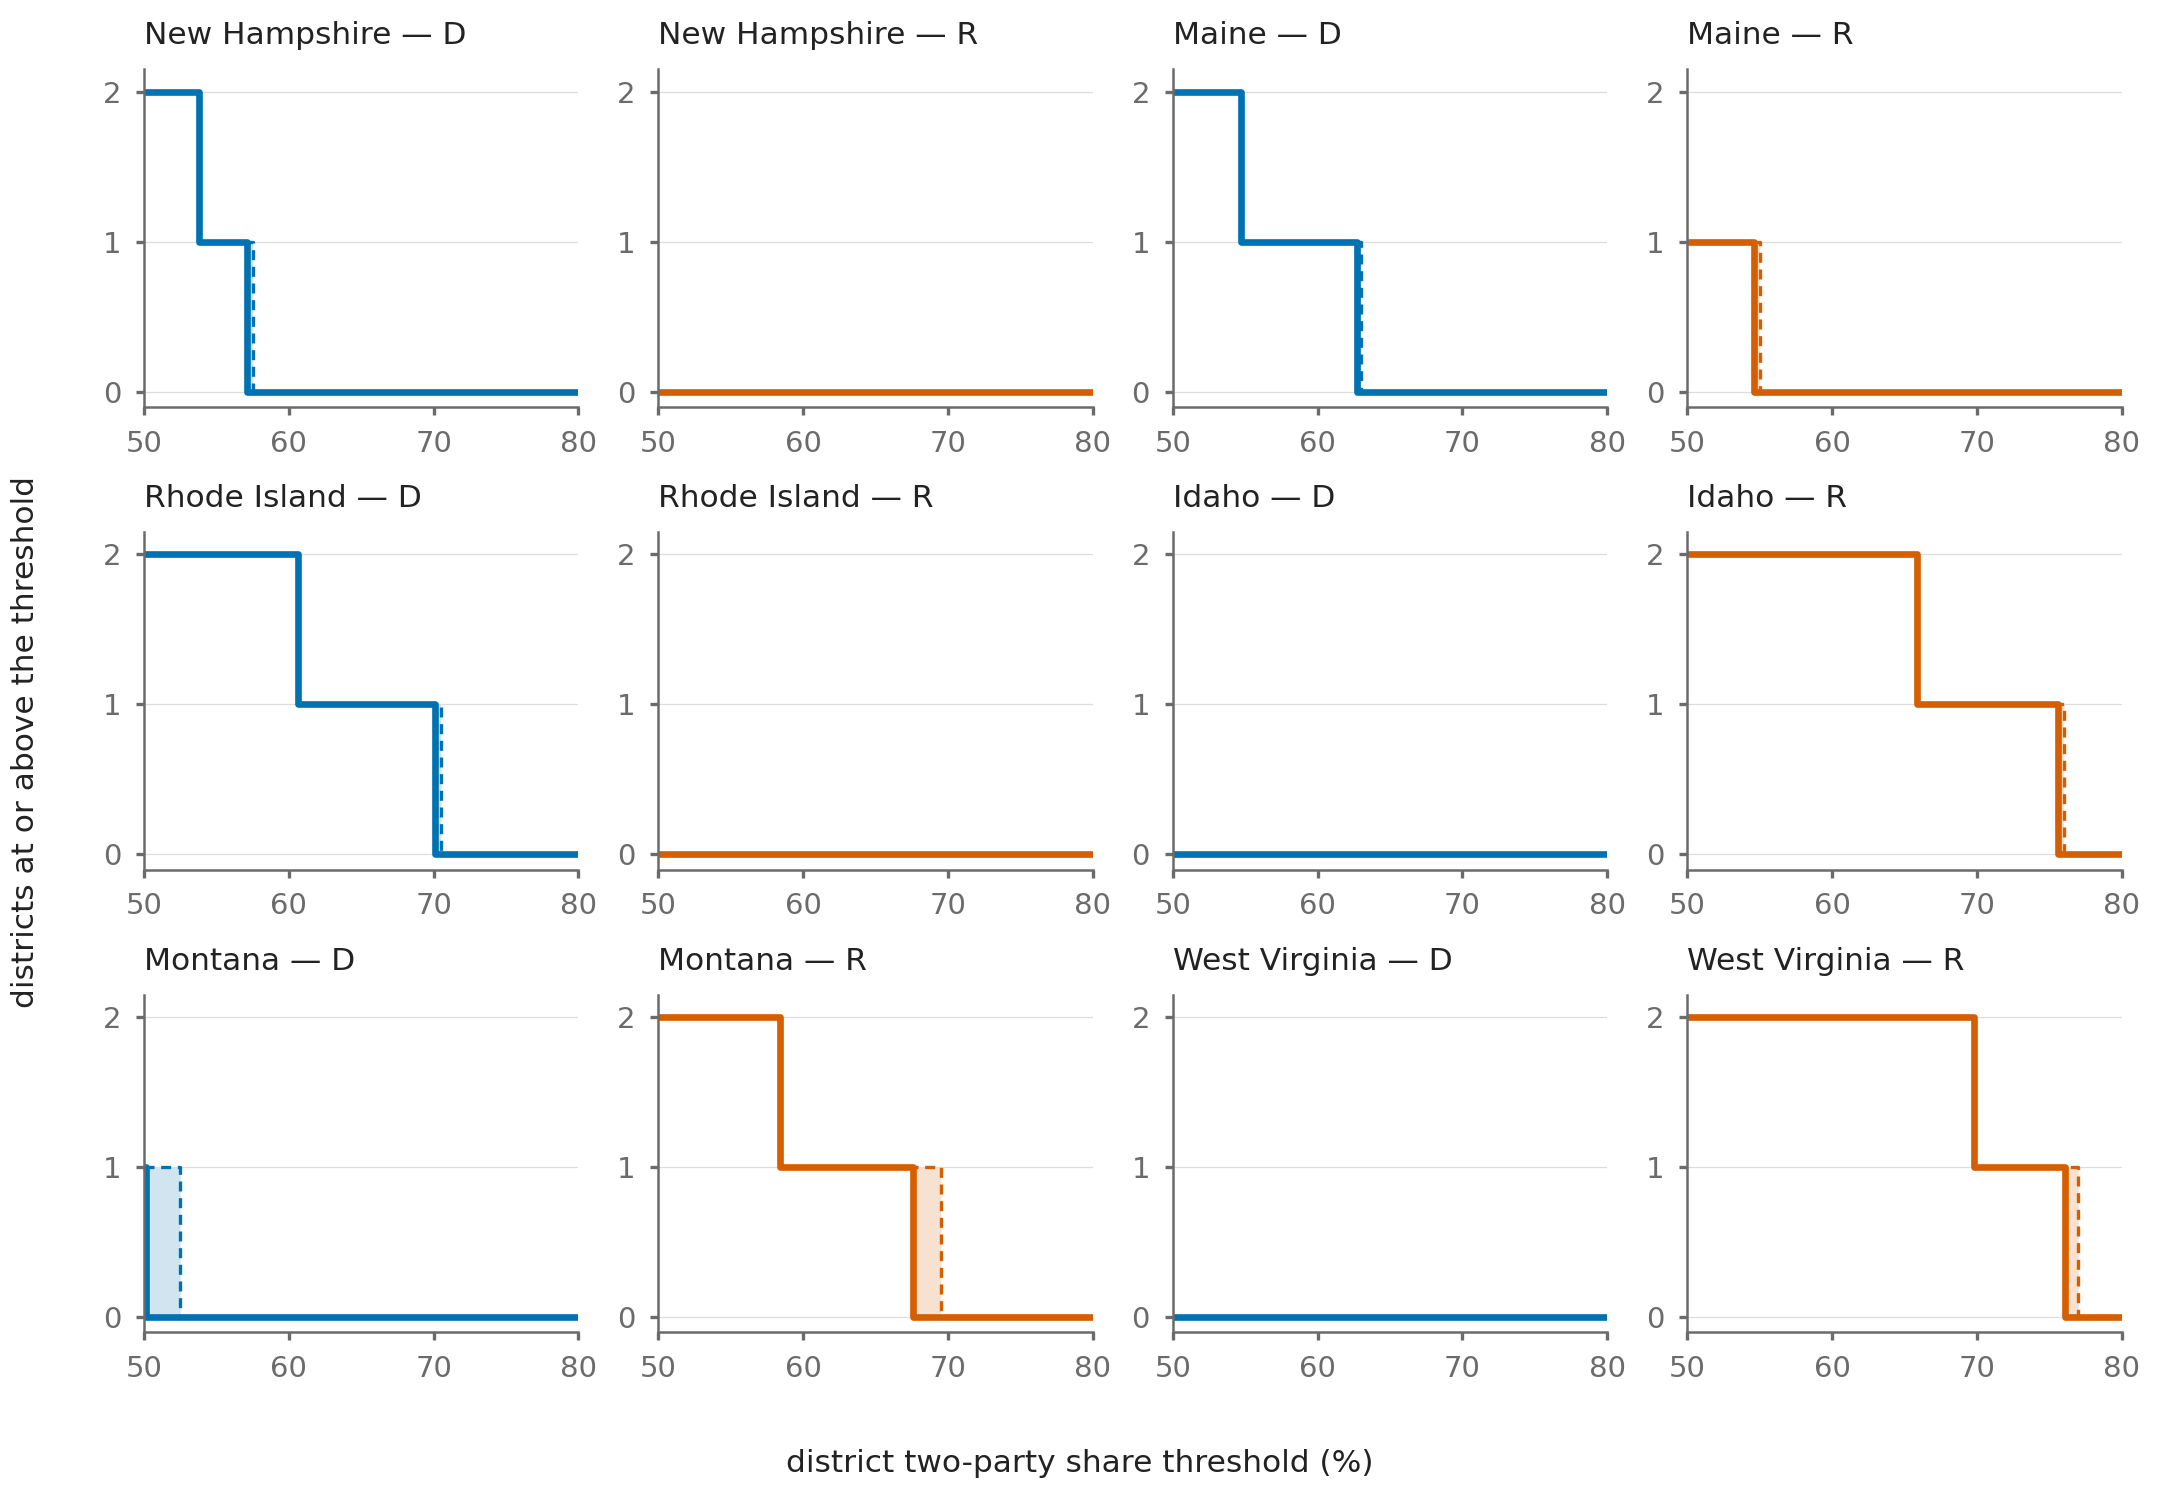
\includegraphics[width=\linewidth]{figs/frontier_k2.png}
\caption{Certified seat--safety frontiers $F(m)$ for the two-district states, both parties. Solid: certified lower staircase (independently verified plans); dashed: certified upper staircase (infeasibility proofs); shading: unresolved band. A party with no line above zero cannot make a district of that share in any plan of the regime.}\label{fig:frontier2}
\end{figure}

\paragraph{Exactness.}
At the three thresholds of Table~\ref{tab:capacity}, 79 of the 96 values of $F$ are pinned exactly: all 36 in the two-district states and 43 of the 60 in the states with three to five districts. Over a one-point grid of thresholds from 50\% to 80\%, 80\% of the 992 (state, party, threshold) values are exact. In terms of the spectrum (Table~\ref{tab:tightness}), 21 of the 24 brackets in the two-district states are tight to half a point of district share (median width 0.01 point once the geography-free bound is used as an additional upper bound) and the median bracket for $3\le k\le5$ is 2.2--2.6 points wide; the widest open brackets (9--14 points) are those of a party that is a minority in a state with three or more districts (Mississippi and Arkansas Democrats at $q=2$, Connecticut Democrats at $q=1$, Mississippi Republicans at $q=2$, Oklahoma Democrats).

\begin{table}[!tbp]
\centering\small
\caption{Width of the certified brackets $[r_q,u_q)$ for $\sigma^*(q)$, in points of district share, by number of districts $k$. Brackets proving that no $q$ districts can reach 50\% count as exact.}\label{tab:tightness}
\adjustbox{max width=\linewidth}{\begin{tabular}{crrrrrr}
\toprule
$k$ & brackets & exact ($\le0.5$ pt) & $\le1$ pt & $\le2$ pt & $\le3$ pt & median width (pts) \\
\midrule
2 & 24 & 21 & 22 & 23 & 24 & 0.01 \\
3 & 12 & 4 & 5 & 6 & 9 & 2.23 \\
4 & 48 & 10 & 12 & 19 & 27 & 2.62 \\
5 & 20 & 9 & 9 & 10 & 13 & 2.21 \\
\bottomrule
\end{tabular}
}
\end{table}

\paragraph{What the exact values say.}
(i) \emph{Certified zeros.} Republicans in New Hampshire and Rhode Island and Democrats in Idaho and West Virginia provably cannot make even one majority district (for Rhode Island, Idaho and West Virginia the geography-free bound already shows it; for New Hampshire Republicans it needs geography: the hull bound allows up to 54.6\%). (ii) \emph{Packing gains.} The best single district of a party can be far above the party's statewide share (Figure~\ref{fig:scatter}): for example Idaho Republicans (65.9\% statewide) can reach 75.5--76.0\%, Rhode Island Democrats (60.6\%) 70.0--70.5\%, and Maine Democrats (54.7\%) 62.7--63.0\% (Figure~\ref{fig:maps} shows witness plans for three of these states). (iii) \emph{The all-safe end is pinned by the statewide share.} Because the turnout-weighted mean of the district margins equals the statewide margin, $\sigma^*(k)$ cannot exceed it, and the resolved certified values sit within 0.2 point of it (Idaho Republicans $q=2$: 65.88\% against 65.9\%; Nebraska Republicans $q=3$: 59.71\% against 59.8\%; Connecticut Democrats $q=5$: 60.12\% against 60.2\%). (iv) \emph{A one-seat statement with geography.} Connecticut Republicans (39.8\% statewide) can make exactly one district with at least 50\%, and none with at least 55\%.

\begin{figure}[!tbp]
\centering
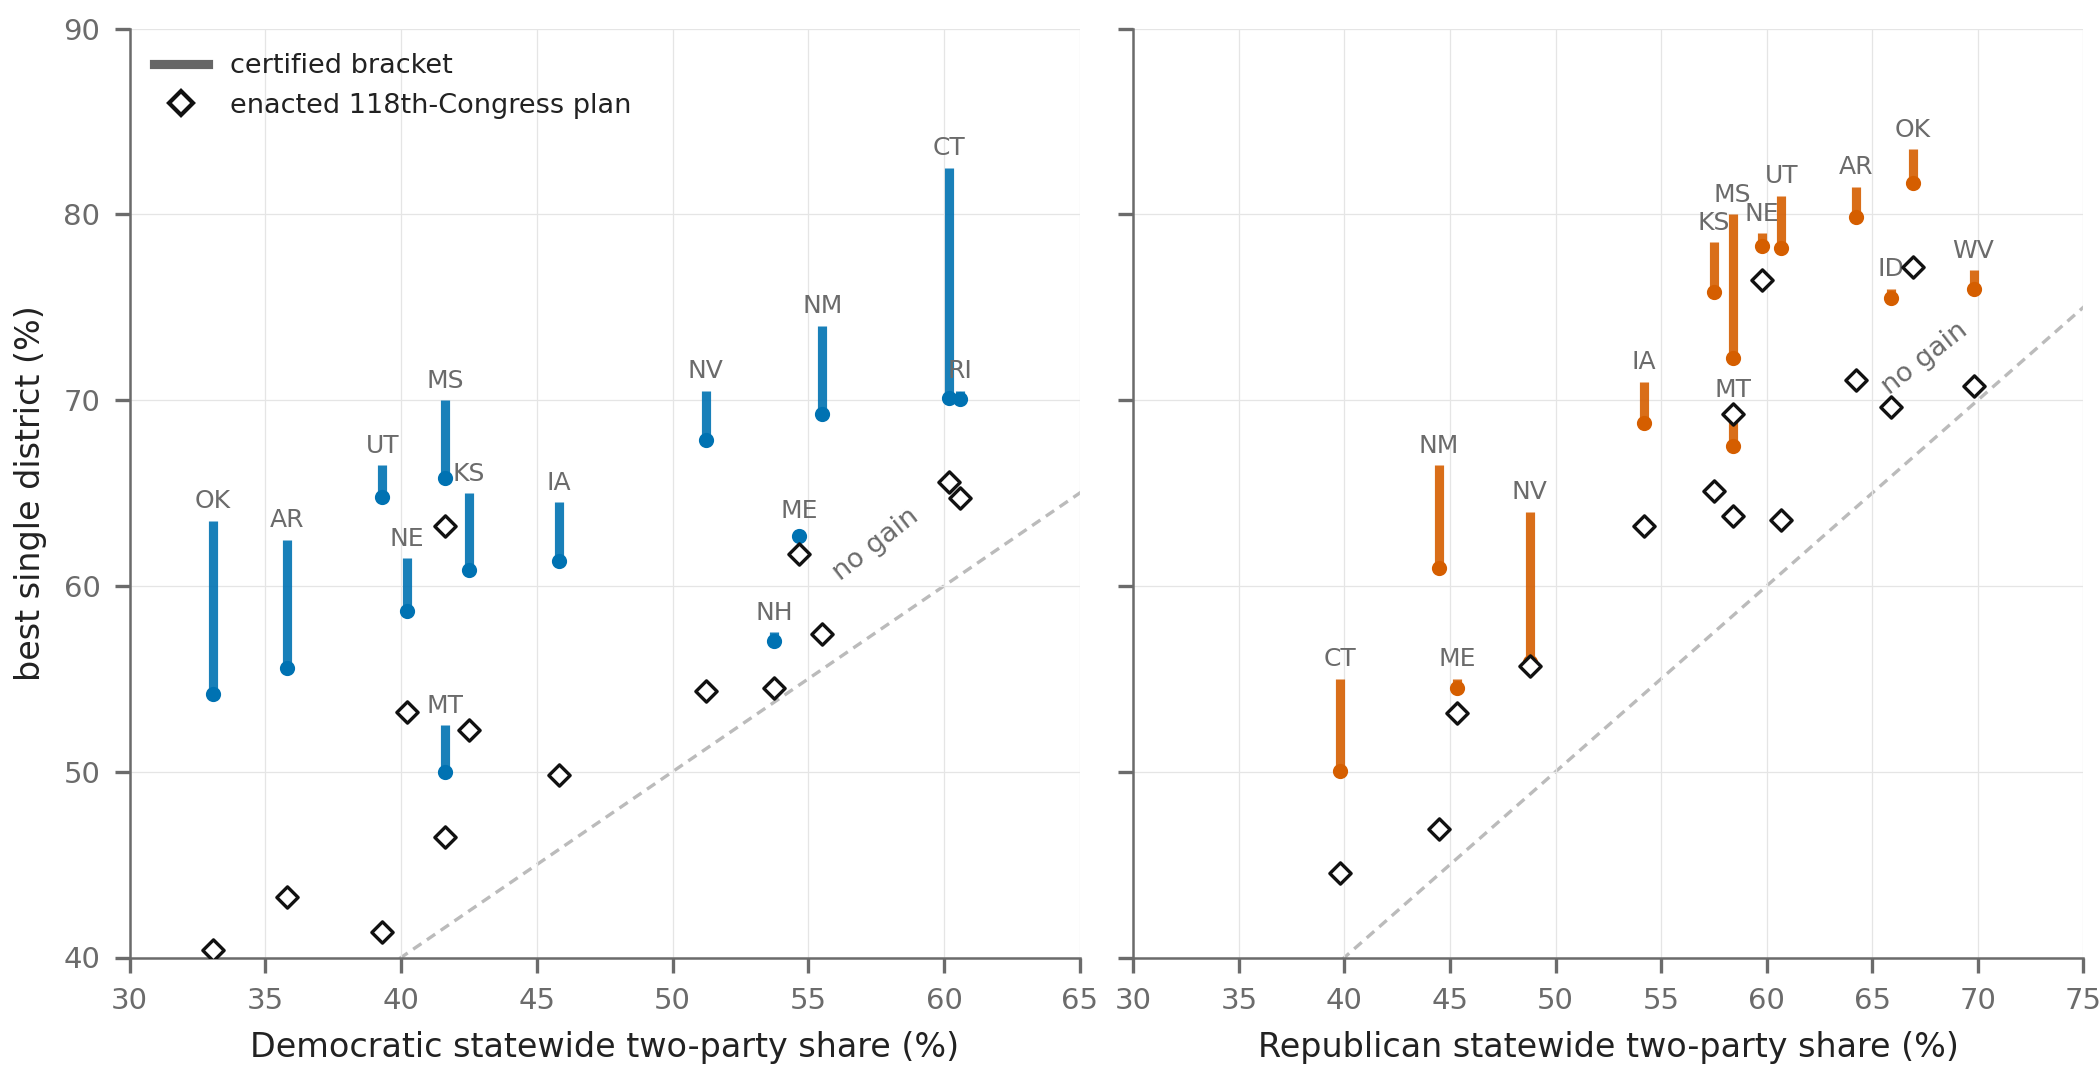
\includegraphics[width=\linewidth]{figs/scatter.png}
\caption{Certified bracket for the best single district ($q=1$) against the party's statewide two-party share. Points on the dashed diagonal would mean the boundaries give no gain.}\label{fig:scatter}
\end{figure}

\begin{figure}[!tbp]
\centering
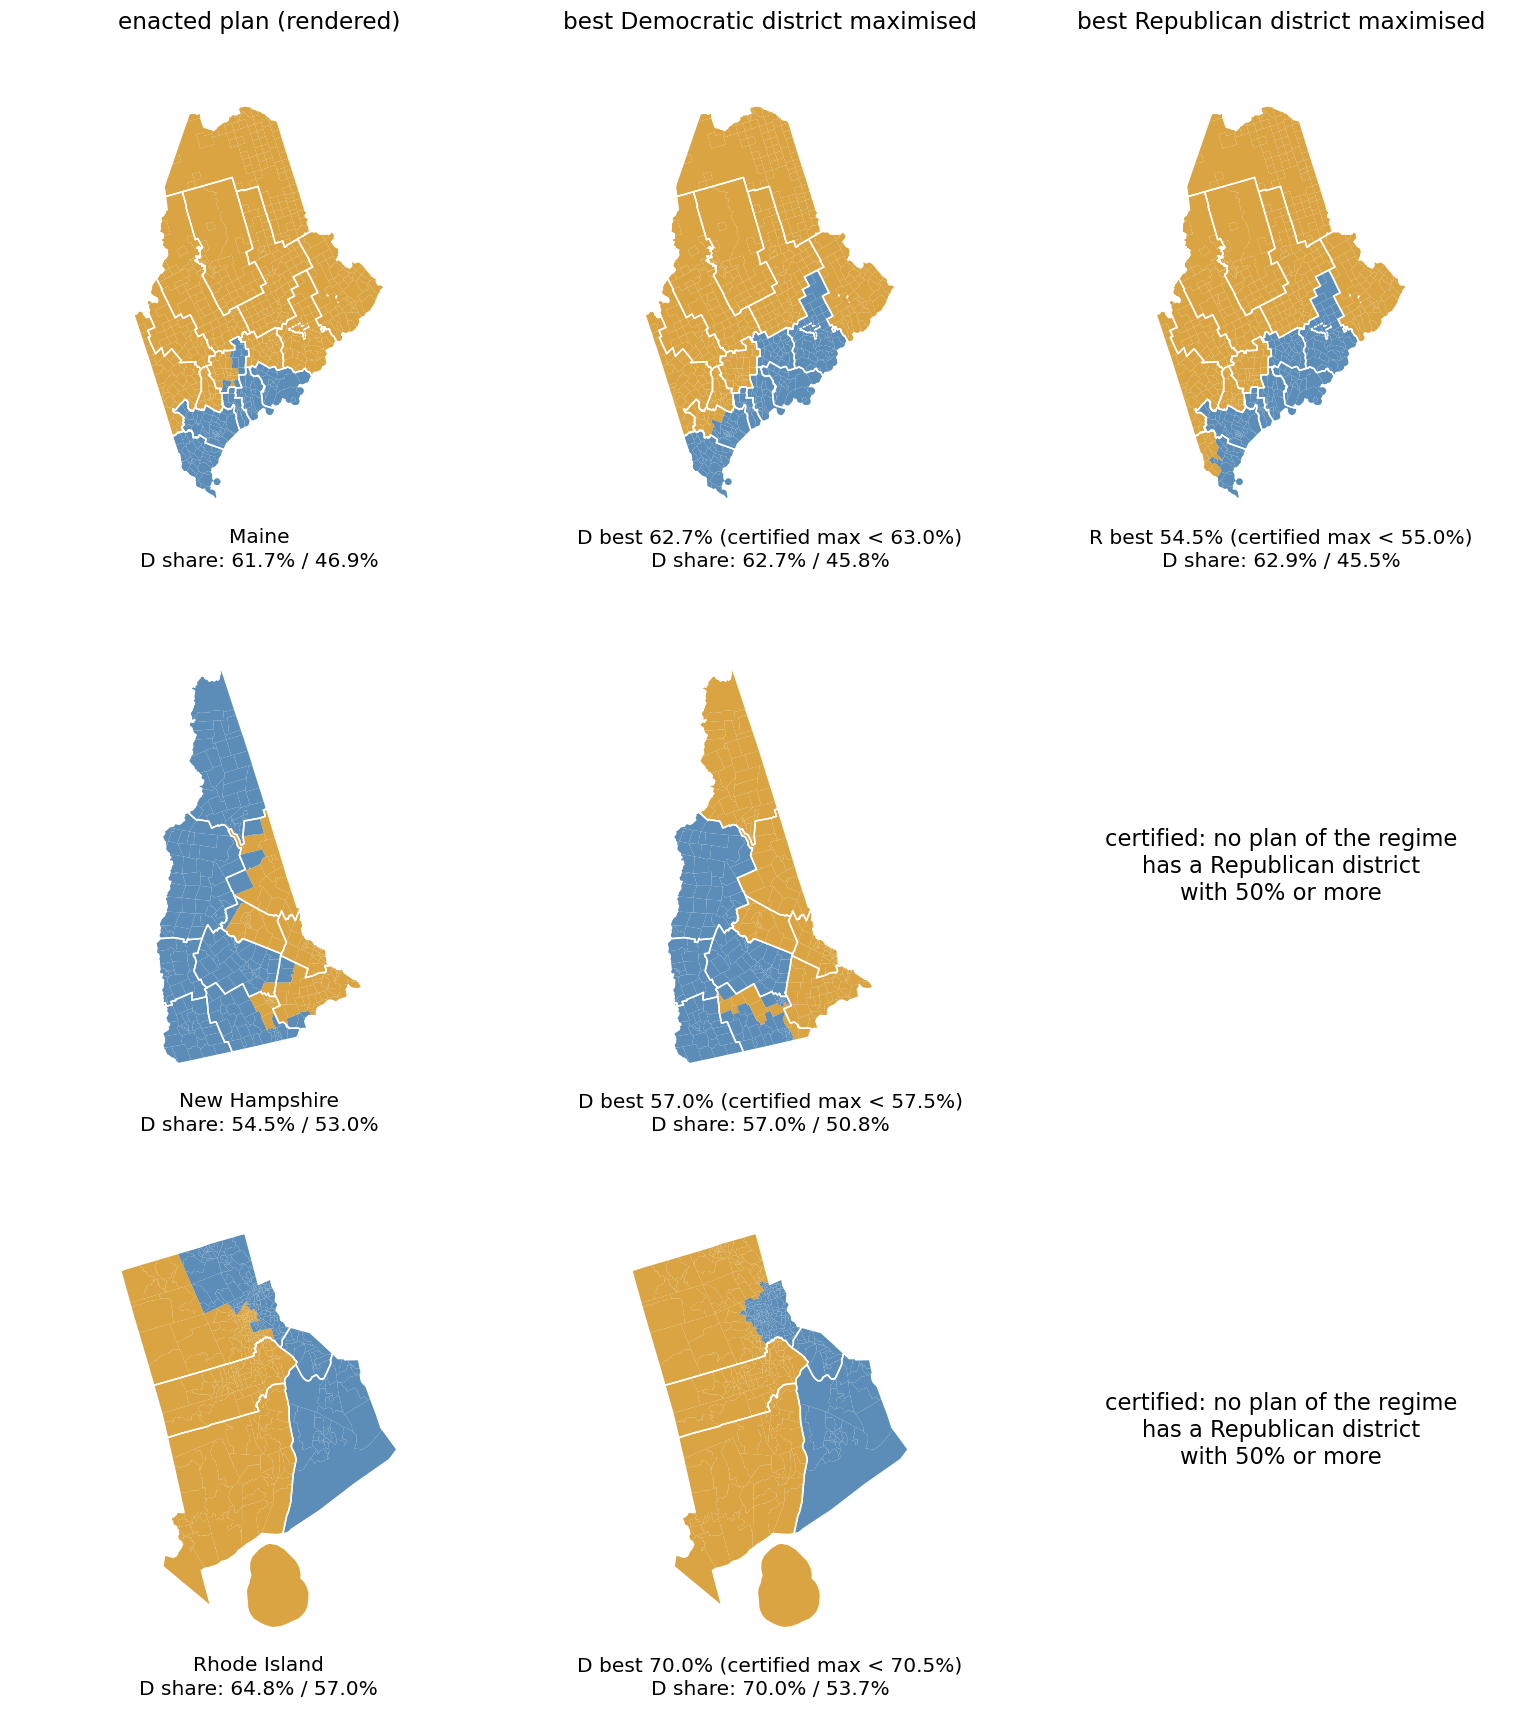
\includegraphics[width=0.9\linewidth,height=0.74\textheight,keepaspectratio]{figs/maps.png}
\caption{Witness plans of the certified brackets for Maine, New Hampshire and Rhode Island (two districts each). Left: the enacted plan rendered at precinct resolution. Middle and right: stored, independently verified plans that maximise the best Democratic (middle) and Republican (right) district; the certified upper end for the same quantity is in the panel title, so each plan is within the bracket width of the true optimum of the regime $\rho_s$. Where the proofs show that a party cannot reach 50\% in any district, no map is shown. Colours identify the district with the higher (blue) and lower (orange) Democratic share, not a party; white lines are county boundaries. These are witnesses that make the lower bounds checkable, not proposals.}\label{fig:maps}
\end{figure}

\begin{figure}[p]
\centering
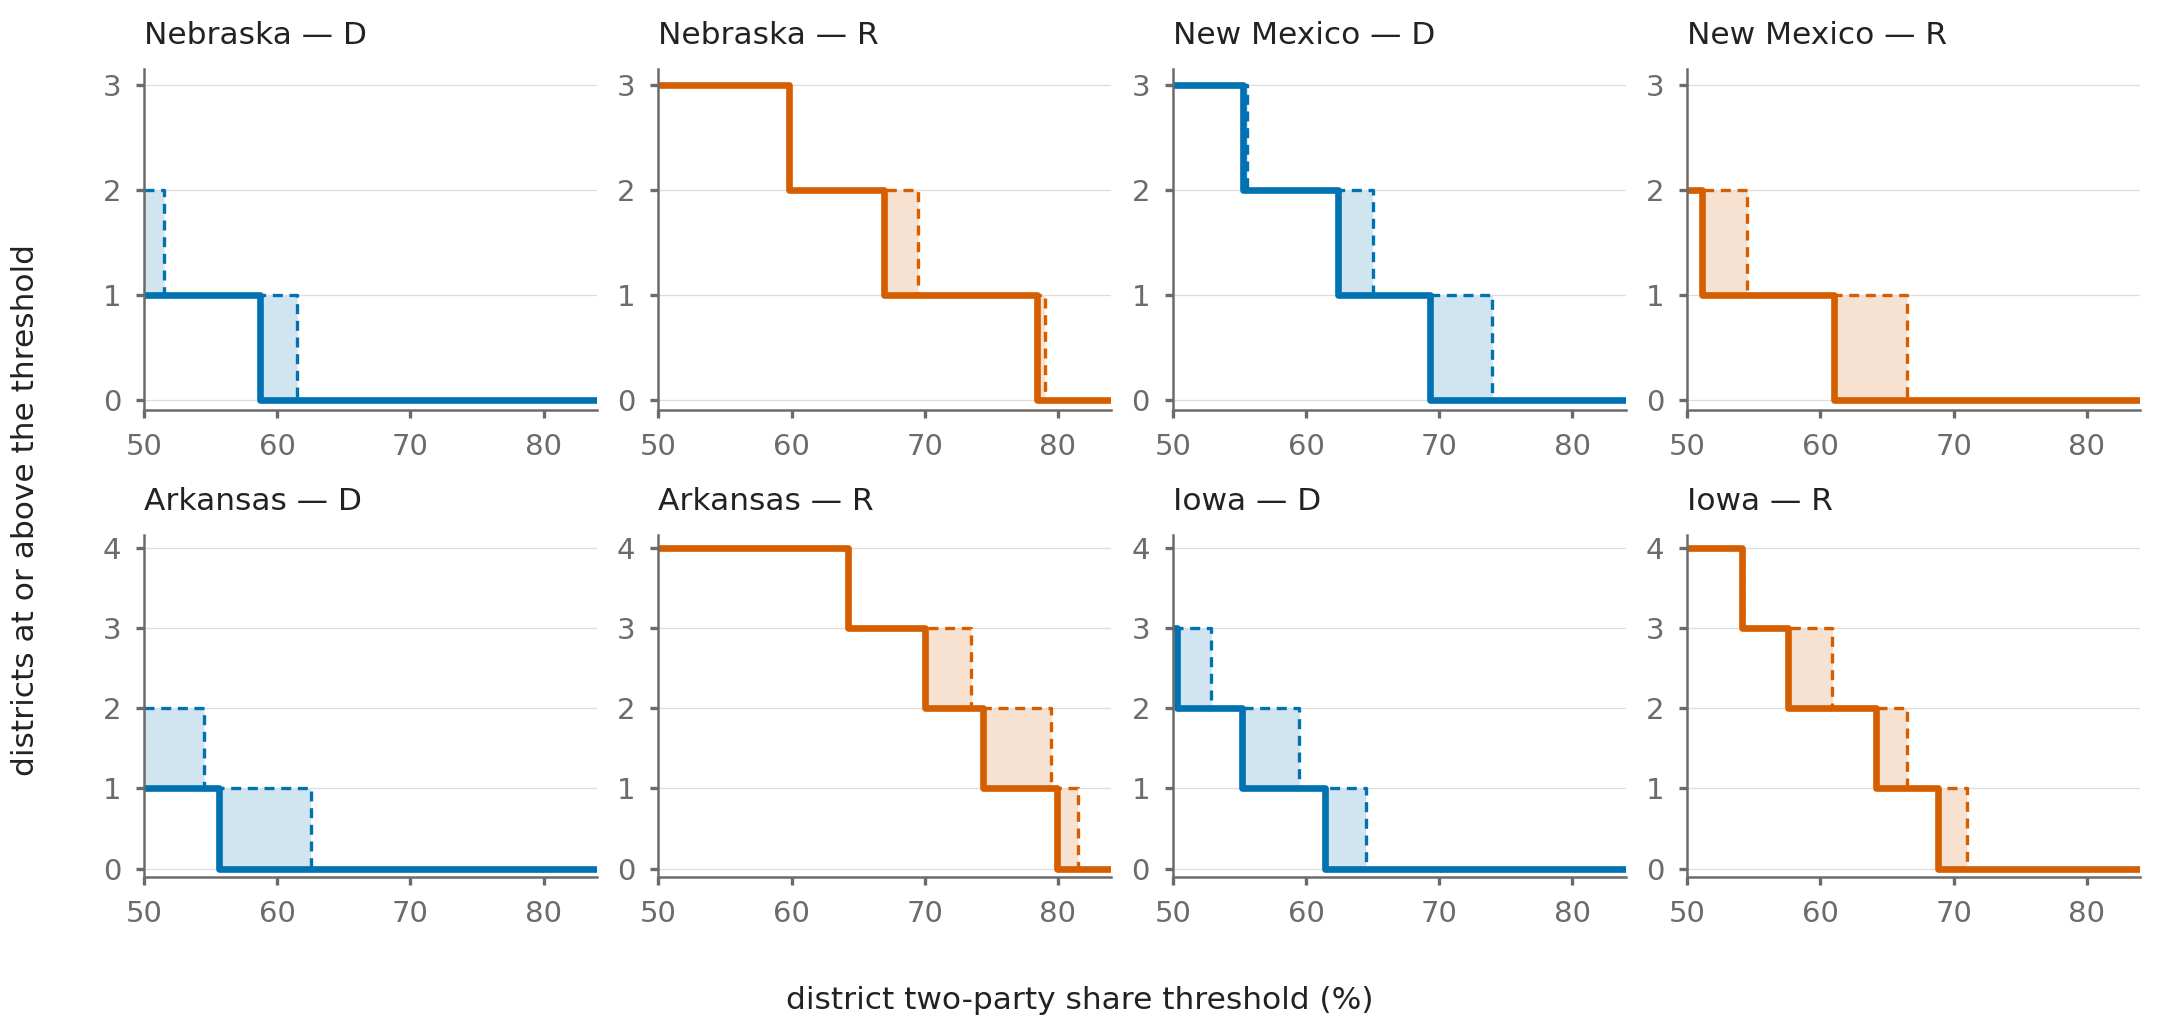
\includegraphics[width=\linewidth]{figs/frontier_k34a.png}\\[4pt]
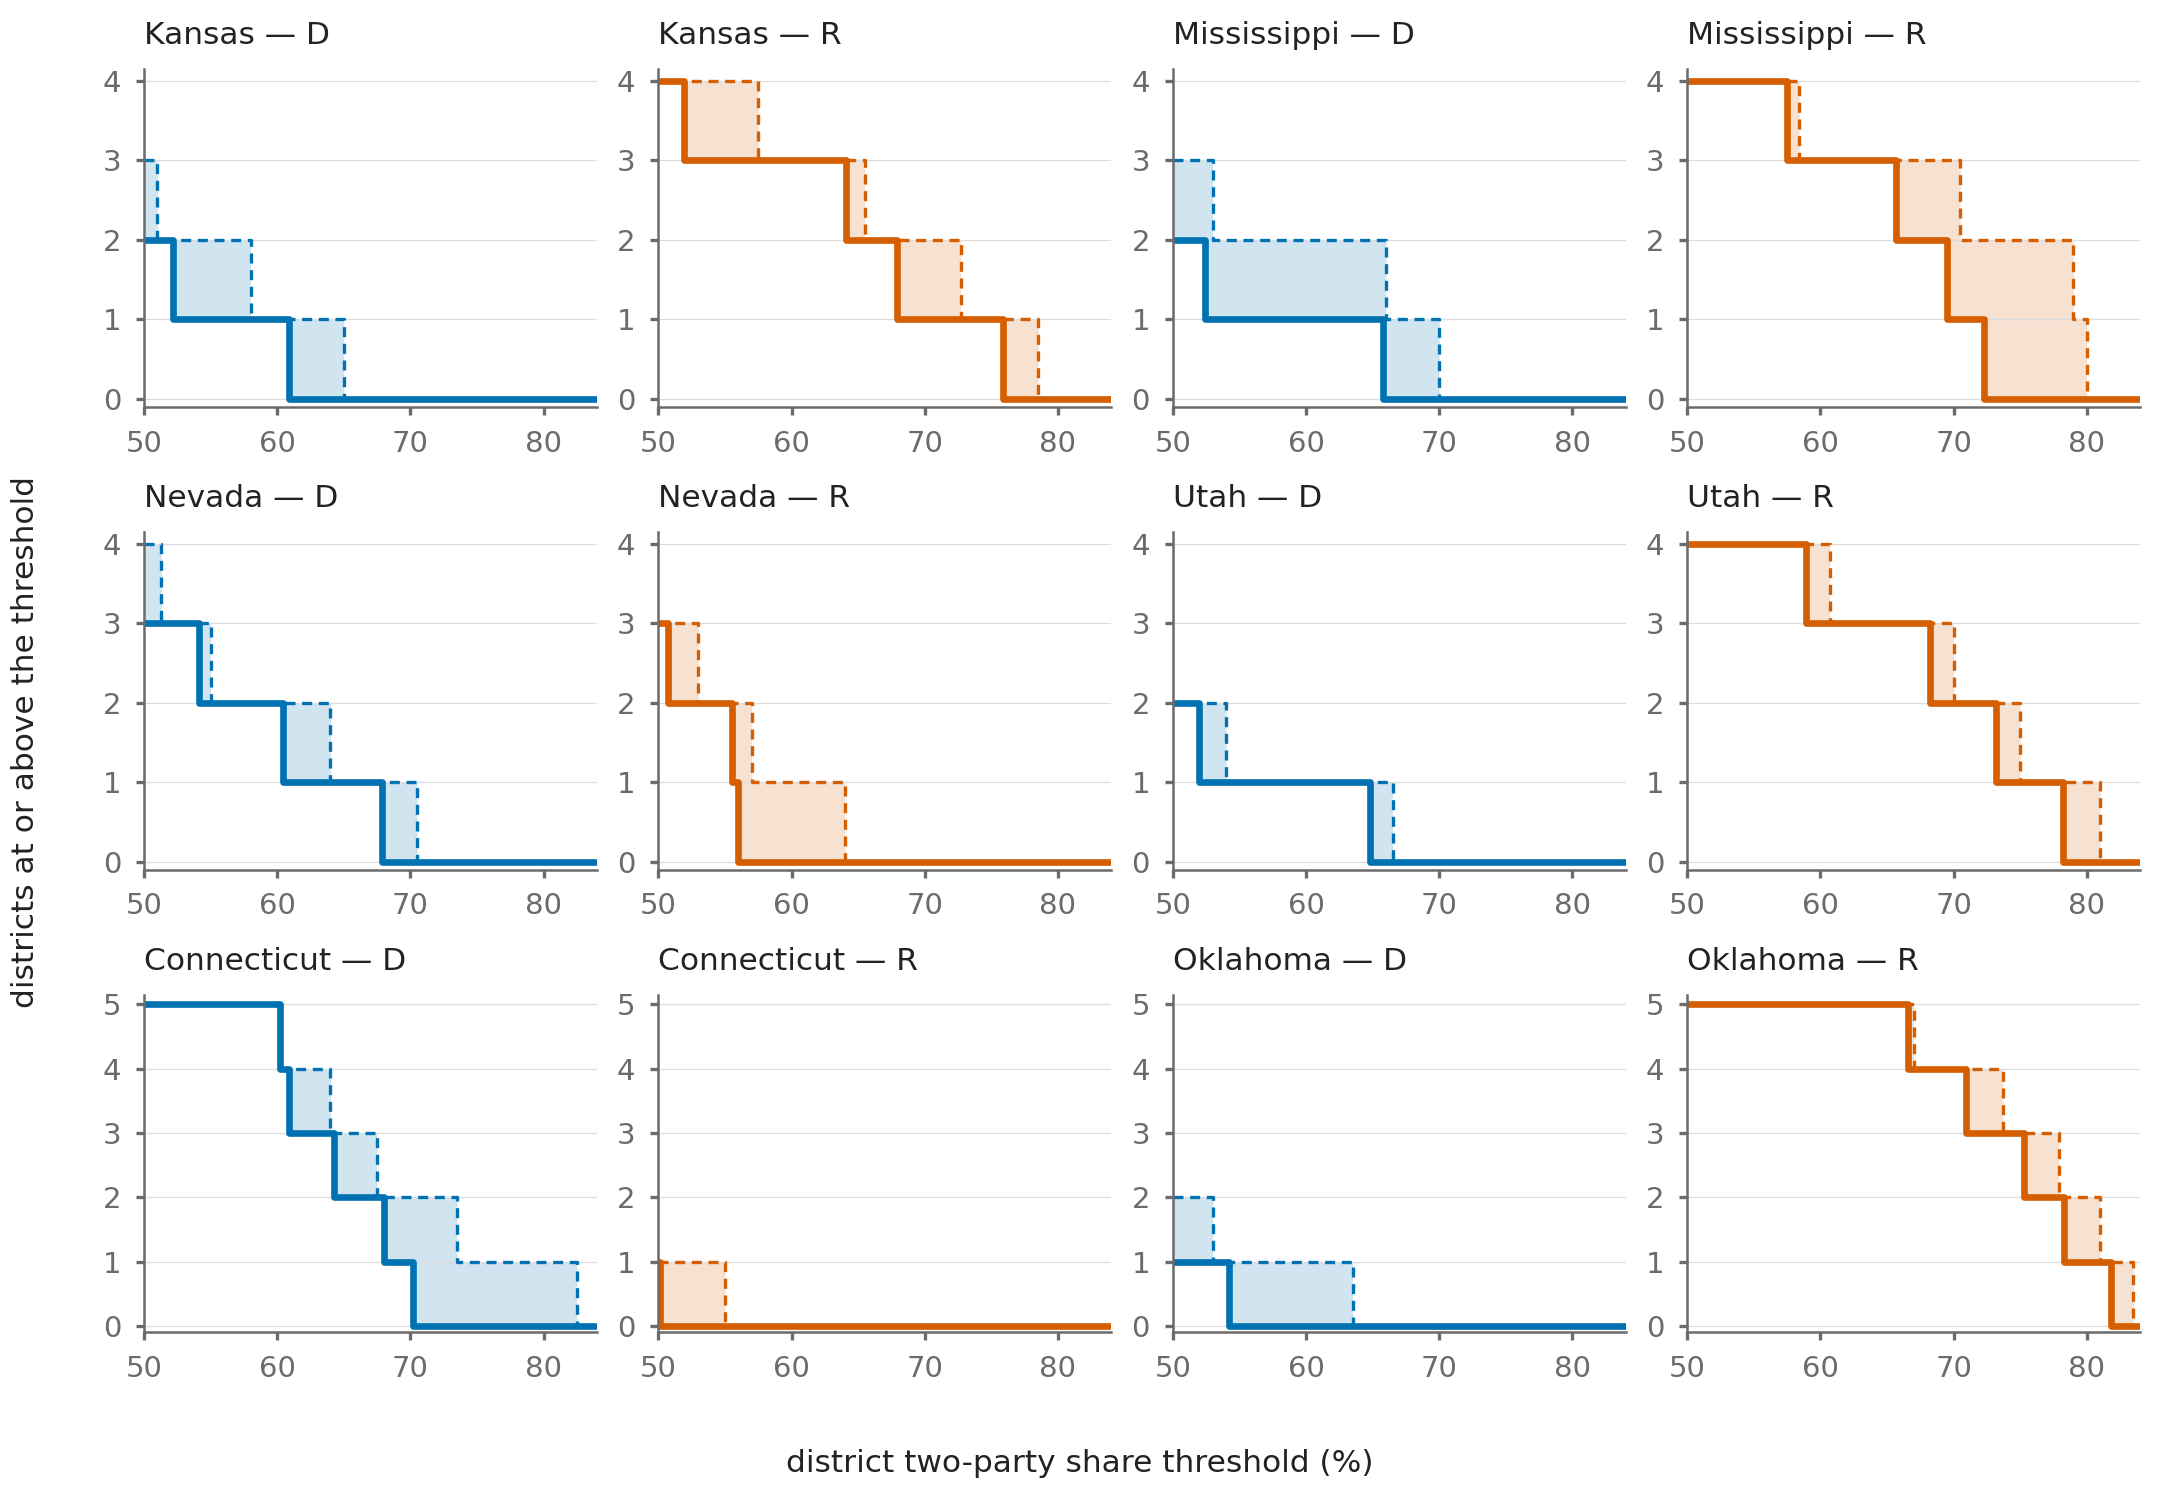
\includegraphics[width=\linewidth]{figs/frontier_k345b.png}
\caption{As Figure~\ref{fig:frontier2} for the states with three to five districts. Shaded bands mark brackets that remain open after the time limits of Section~\ref{sec:results}.}\label{fig:frontier3}
\end{figure}


\subsection{Seat ranges and the enacted plans in context}\label{sec:enacted}

The frontier at threshold $50\%$ has a direct seat interpretation. With two-party shares a district is Democratic-majority exactly when it is not Republican-majority, so under a regime $\rho$ the number of Democratic-majority districts of any plan lies between $k-F^{R}_\rho(0)$ and $F^{D}_\rho(0)$, and both ends are attained by some plan (Proposition~\ref{prop:mono}(4) gives the Republican side from the same code). Certified bounds on $F^D$ and $F^R$ therefore give a certified \emph{seat range} for each state; Table~\ref{tab:enacted} and Figure~\ref{fig:seatrange} report it next to the delegation of the enacted 118th-Congress plan and the seat count that would be proportional to the statewide vote. All counts use the two-party 2020 presidential vote in each district; they are descriptions of vote geography, not predictions of congressional results. (A district with an exactly tied two-party vote would count for both parties at threshold 50\%, so the range is exact up to such ties.)

\begin{table}[!tbp]
\centering\footnotesize
\caption{Seat range under $\rho_s$ at threshold 50\% and the enacted plans (2022 elections; each rendered at precinct resolution, Section~\ref{sec:data}). Columns give numbers of Democratic-majority districts: ``enacted'' for the enacted plan; ``verified'' the smallest and largest count attained by independently verified plans of $\rho_s$; ``limits'' what the infeasibility proofs leave possible. Splits are $\sum_K(d_K-1)$ of the rendered plan with the budget $s$ of $\rho_s$ in parentheses; ``in $\rho_s$'' says whether the rendered plan satisfies $\rho_s$ (population within $\pm1\%$, connected, at most $k-1$ splits).}\label{tab:enacted}
\adjustbox{max width=\linewidth}{\begin{tabular}{lrrcccrrc}
\toprule
State & $k$ & D share & enacted & verified & limits & splits ($s$) & max.\ dev. & in $\rho_s$ \\
\midrule
New Hampshire & 2 & 53.7\% & 2 & 2 & 2 & 5 (1) & 0.00\% & no \\
Maine & 2 & 54.7\% & 1 & 1--2 & 1--2 & 1 (1) & 0.00\% & yes \\
Rhode Island & 2 & 60.6\% & 2 & 2 & 2 & 1 (1) & 0.19\% & yes \\
Idaho & 2 & 34.1\% & 0 & 0 & 0 & 1 (1) & 0.02\% & yes \\
Montana & 2 & 41.6\% & 0 & 0--1 & 0--1 & 1 (1) & 0.07\% & no \\
West Virginia & 2 & 30.2\% & 0 & 0 & 0 & 0 (1) & 0.09\% & yes \\
Nebraska & 3 & 40.2\% & 1 & 0--1 & 0--2 & 2 (2) & 0.37\% & yes \\
New Mexico & 3 & 55.5\% & 3 & 1--3 & 1--3 & 10 (2) & 0.64\% & no \\
Arkansas & 4 & 35.8\% & 0 & 0--1 & 0--2 & 3 (3) & 0.05\% & yes \\
Iowa & 4 & 45.8\% & 0 & 0--3 & 0--3 & 0 (3) & 0.01\% & yes \\
Kansas & 4 & 42.5\% & 1 & 0--2 & 0--3 & 4 (3) & 0.05\% & no \\
Mississippi & 4 & 41.6\% & 1 & 0--2 & 0--3 & 4 (3) & 0.12\% & no \\
Nevada & 4 & 51.2\% & 3 & 1--3 & 1--4 & 3 (3) & 0.36\% & yes \\
Utah & 4 & 39.3\% & 0 & 0--2 & 0--2 & 7 (3) & 0.76\% & no \\
Connecticut & 5 & 60.2\% & 5 & 4--5 & 4--5 & 10 (4) & 0.77\% & no \\
Oklahoma & 5 & 33.1\% & 0 & 0--1 & 0--2 & 7 (4) & 0.21\% & no \\
\bottomrule
\end{tabular}
}
\end{table}

\begin{figure}[!tbp]
\centering
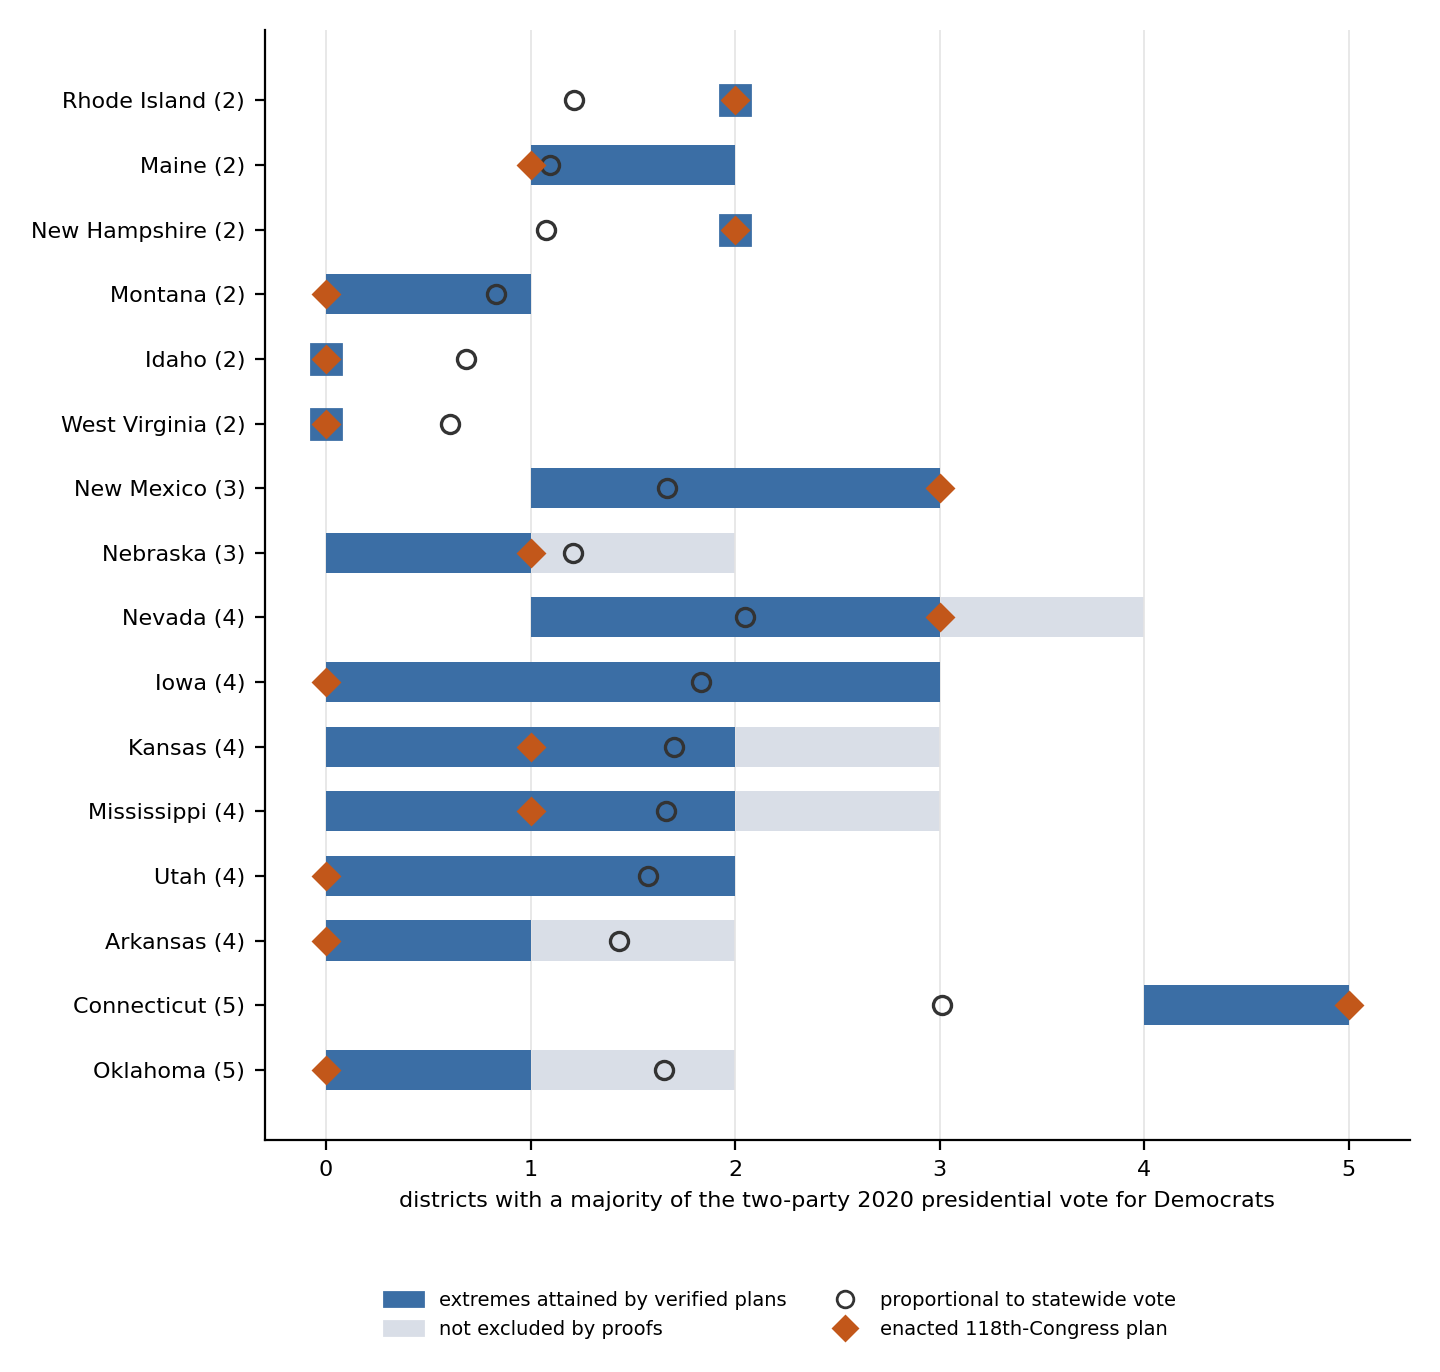
\includegraphics[width=0.86\linewidth,height=0.6\textheight,keepaspectratio]{figs/seatrange.png}
\caption{Certified range of the number of Democratic-majority districts under $\rho_s$ (threshold 50\% of the two-party 2020 presidential vote), the delegation of the enacted plan, and proportionality. Both extremes of the dark bar are attained by verified plans; light grey marks counts that the proofs do not exclude. Intermediate counts are not claimed to be attained.}\label{fig:seatrange}
\end{figure}

\paragraph{Where line drawing decides and where geography does.}
In four of the 16 states (New Hampshire and Rhode Island for Democrats, Idaho and West Virginia for Republicans) the delegation is the same for every plan of $\rho_s$: the two ends of the certified range coincide (Table~\ref{tab:enacted}). In the other twelve, verified plans attain a spread of one to three seats, and the proofs leave at most one further seat open in six of them; summed over the 52 seats of the 16 states, verified plans move the Democratic count between $11$ and $30$ and the proofs exclude anything below $11$ or above $36$ (the separability of Proposition~\ref{prop:sep} makes such sums valid for the union of states). Verified plans give Republicans a majority of the delegation in twelve of the 16 states and Democrats in seven; Iowa, Nevada and New Mexico are in both lists, and in New Hampshire, Rhode Island, Maine and Connecticut only Democrats can (in Maine Republicans can hold at most one of the two seats). Both parties are run through identical code, so which side has this capacity is a property of each state's vote geography and the regime. The Democratic delegations of the enacted plans total 19 of 52 seats (proportionality to the statewide votes would give 23.3), inside the verified range of 11 to 30.

\paragraph{The enacted plans in context.}
The rendered enacted plans are outside the regime in eight states, mainly because they split more counties than $k-1$ (Table~\ref{tab:enacted}; Montana's rendering has one detached precinct of 530 residents), and were drawn under criteria our model does not include, so their position relative to the range is a description and no evidence about intent. With that caveat, three observations are certified. First, in each of the 71 (state, party, $q$) combinations for which a verified plan has a $q$-th district above 50\%, the $q$-th best district of the enacted plan is below the certified lower end of $\sigma^*(q)$: by a median of 5.9 points of district share (5.4 points for the 28 single-best-district cases; smallest gap 0.2, largest 23.4; Figure~\ref{fig:scatter}, diamonds). No enacted plan exhausts what boundaries could do for either party at any rank, although a single plan cannot exhaust all ranks at once. Second, the delegation of the enacted plan lies at an end of the verified seat range in ten of the twelve states in which the range is not a single value, and in the interior in two (Kansas and Mississippi, each with one Democratic seat in a verified range of $0$--$2$); the end is the Republican end (fewest Democratic seats) in six of the ten and the Democratic end in four. Third, the enacted plans supply an independent test of the bounds: the eight of them that satisfy $\rho_s$ are ordinary plans of the regime, shaped by others (the test concerns the rendered plans, which are verified plans of $\rho_s$ whatever their fidelity to the enacted maps), and none of their 46 (party, $q$) margins reaches the proven upper end of the corresponding bracket, while none exceeds a lower end, so no plan in the public record improves our lower bounds in these states.


\subsection{Why the budget matters: connectivity coarsening alone does not help}\label{sec:negative}

The relaxation of Section~\ref{sec:relax} has two ingredients that can each tighten the geography-free bound: connectivity of the cell support in the quotient graph, and the subdivision budget. To separate them we ran, for every (state, party, $q$), (a) the geography-free hull bound (one cell, no connectivity: the sorting bound of \citealt{duchin2019}, extended to $k$-way allocations and the whole spectrum), (b) the aggregated relaxation with counties as cells and connectivity but \emph{no budget}, (c) the same after two uniform levels of refinement (roughly four to ten times as many cells), and compared them with the certified bracket under the budget $s=k-1$ (Figure~\ref{fig:ablation}, Table~\ref{tab:ablation} in the appendix; for $k\ge3$ the relaxations (a)--(c) are the pool relaxations with one aggregate for the unsafe districts, which are also valid).

\begin{figure}[!tbp]
\centering
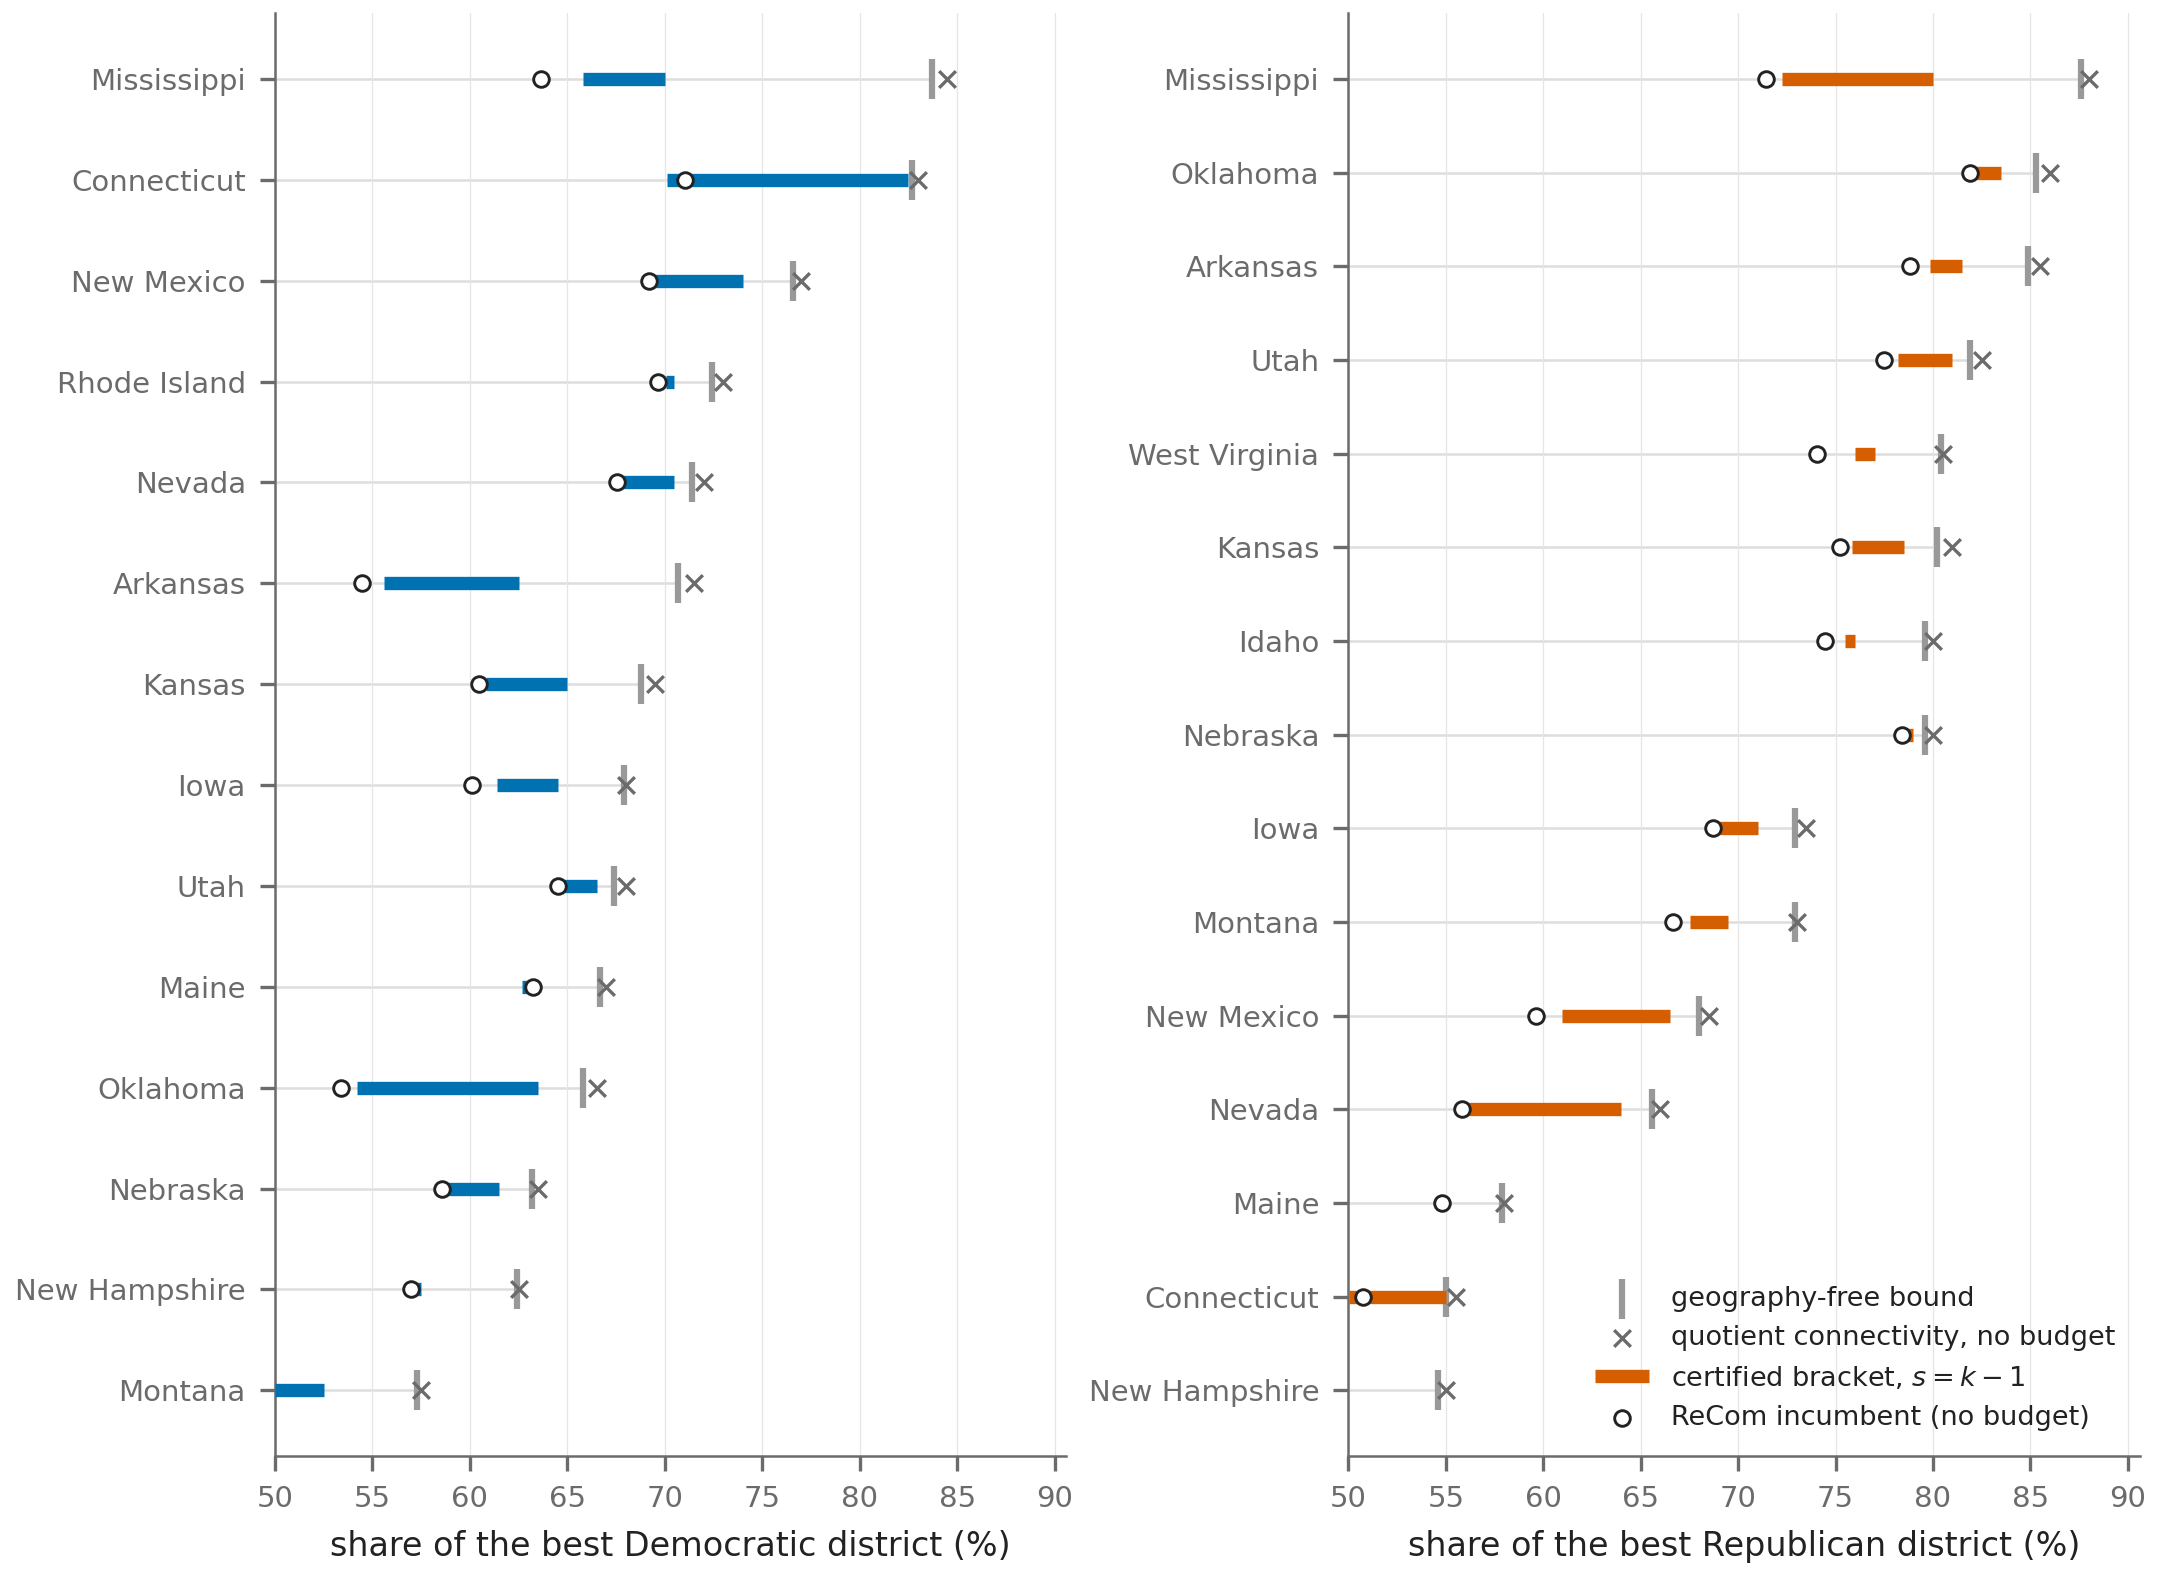
\includegraphics[width=\linewidth,height=0.68\textheight,keepaspectratio]{figs/ablation.png}
\caption{Upper bounds and incumbents for the share of the most extreme district ($q=1$), states with a nontrivial bound. Grey bar: geography-free hull bound; cross: quotient-connectivity relaxation with counties as cells and no budget (identical to within grid resolution after two further refinement levels); circle: 40-second unconstrained ReCom hill-climbing incumbent; thick bar: certified bracket under the budget of $k-1$ county splits.}\label{fig:ablation}
\end{figure}

\paragraph{Connectivity coarsening alone does nothing.}
Over the 79 nontrivial (state, party, $q$) triples the quotient relaxation without budget is never tighter than the geography-free bound (difference $+0.3$ point at the median, range 0.0 to $+0.8$, i.e. grid noise), and neither is it after two levels of refinement. This is the phenomenon of Proposition~\ref{prop:blind}: a district can touch every cell of a connected cell set while taking, in each cell, exactly its best atoms.

\paragraph{The budget does.}
The certified upper end under the budget is tighter than the geography-free bound by more than 0.05 point in 55 of the 78 triples with a finite upper end (median improvement 0.65 point; for $q=1$ the median is 2.75 points with a range from 0.2 to 13.7 points). Where it is not, the bracket is one of the open ones (Section~\ref{sec:main}) and the geography-free bound is used as the upper end (Table~\ref{tab:spectrum}). For the two-district states the improvement is decisive: New Hampshire Democrats 62.4\% $\to$ 57.0--57.5\%, Idaho Republicans 79.6\% $\to$ 75.5--76.0\%, West Virginia Republicans 80.4\% $\to$ 76.0--77.0\%.

\paragraph{Counting by pieces.}
Counting split \emph{counties} instead of pieces (a county cut among all districts costs one split) leaves a whole county as an unconstrained sub-problem. In development this was visible in Nebraska, where Douglas County holds 30\% of the state's population: under that convention the relaxed solutions of a query near the transition cut Douglas three ways for a single split, so that the exact problem contained a free three-way partition of 237 precincts, and CP-SAT alone could not even produce a feasible plan for $q=0$ within 300~s (a county-aware recombination heuristic finds one in milliseconds). We therefore adopted the piece-based count, which is also the convention of the exact county-split literature, and report only its results; we did not attempt a controlled comparison of the two conventions.


\subsection{Refinement versus monolithic exact solves}\label{sec:baseline}

Is the refinement loop needed, or would an exact solver on the atomic model do? We posed the 20 decision queries that produce the upper ends of the two-district brackets (for each state, party and rank the tightest margin at which the loop proved infeasibility; Table~\ref{tab:baseline}) to three exact methods under the same regime with a 300-second limit each: the CEGAR loop; CP-SAT on the atomic model of Section~\ref{sec:relax} (every precinct its own cell, exact parent-pointer connectivity and split row); and HiGHS on the independently written single-commodity-flow MILP of Section~\ref{sec:audit} on the atomic partition.

\begin{table}[!tbp]
\centering\footnotesize
\caption{Decision queries (``$q$ districts with share at least $m$?'', all answered ``no'' by the loop) posed to the CEGAR loop and to two monolithic exact solvers on the atomic model, 300 s limit, five CP-SAT workers (HiGHS: default threads). ``proof'' = proved infeasible; ``unknown'' = undecided at the limit. No solver returned a plan for a query that another proved infeasible.}\label{tab:baseline}
\adjustbox{max width=\linewidth}{\begin{tabular}{llcrrrr}
\toprule
State & Party & $q$ & margin $m$ & CEGAR & CP-SAT, atomic & HiGHS MILP, atomic \\
\midrule
Idaho & D & 1 & 50.0\% & proof ($<$1\,s) & proof (6\,s) & proof (2\,s) \\
Idaho & R & 1 & 76.0\% & proof (19\,s) & unknown ($>$300\,s) & unknown ($>$300\,s) \\
Idaho & R & 2 & 66.0\% & proof ($<$1\,s) & proof (1\,s) & proof (2\,s) \\
Maine & D & 1 & 63.0\% & proof ($<$1\,s) & proof (19\,s) & proof (41\,s) \\
Maine & D & 2 & 55.0\% & proof ($<$1\,s) & proof ($<$1\,s) & proof ($<$1\,s) \\
Maine & R & 1 & 55.0\% & proof ($<$1\,s) & proof (5\,s) & proof (2\,s) \\
Maine & R & 2 & 50.0\% & proof ($<$1\,s) & proof ($<$1\,s) & proof (1\,s) \\
Montana & D & 1 & 52.5\% & proof (91\,s) & unknown ($>$300\,s) & unknown ($>$300\,s) \\
Montana & D & 2 & 50.0\% & proof ($<$1\,s) & proof ($<$1\,s) & proof ($<$1\,s) \\
Montana & R & 1 & 69.5\% & proof (7\,s) & unknown ($>$300\,s) & unknown ($>$300\,s) \\
Montana & R & 2 & 58.5\% & proof ($<$1\,s) & proof (1\,s) & proof (1\,s) \\
New Hampshire & D & 1 & 57.5\% & proof ($<$1\,s) & unknown ($>$300\,s) & unknown ($>$300\,s) \\
New Hampshire & D & 2 & 54.0\% & proof ($<$1\,s) & proof ($<$1\,s) & proof ($<$1\,s) \\
New Hampshire & R & 1 & 50.0\% & proof ($<$1\,s) & unknown ($>$300\,s) & unknown ($>$300\,s) \\
Rhode Island & D & 1 & 70.5\% & proof (52\,s) & proof (19\,s) & unknown ($>$300\,s) \\
Rhode Island & D & 2 & 61.0\% & proof ($<$1\,s) & proof ($<$1\,s) & proof ($<$1\,s) \\
Rhode Island & R & 1 & 50.0\% & proof ($<$1\,s) & proof (1\,s) & proof ($<$1\,s) \\
West Virginia & D & 1 & 50.0\% & proof ($<$1\,s) & proof (11\,s) & proof (5\,s) \\
West Virginia & R & 1 & 77.0\% & proof (197\,s) & unknown ($>$300\,s) & unknown ($>$320\,s) \\
West Virginia & R & 2 & 70.0\% & proof ($<$1\,s) & proof (2\,s) & proof (7\,s) \\
\bottomrule
\end{tabular}
}
\end{table}

The loop decides all 20 (median 0.2 s; the slowest, West Virginia Republicans at 77\%, takes 197 s); atomic CP-SAT decides 14 and atomic HiGHS 13, and no two methods contradict each other, which is also a consistency check on the proofs (a plan returned where the loop proved infeasibility would refute the proof). The monolithic models are fast where the geography-free bound already nearly settles the query (every $q=2$ query and most zero-capacity queries: 0.3--41 s) and fail exactly on the seven best-district ($q=1$) queries near the transition margin, where the answer depends on how a county can be split. The largest contrast is New Hampshire: the county-level relaxation proves in about a tenth of a second (10 cells) that Democrats cannot reach 57.5\% and that Republicans cannot reach 50\% in any district, while neither monolithic solver decides either query in 300 s. The loop is not uniformly faster: atomic CP-SAT decides Rhode Island Democrats at 70.5\% in 19 s against 52 s for the loop. The comparison is between decision procedures under one time limit on one machine, not a statement about the best possible implementation of either.

\paragraph{Without the budget.}
The same test without a county-split budget ($s=\infty$) shows how much of the tractability comes from the budget. For three best-district queries---New Hampshire Democrats at 56\% and 58\%, Maine Democrats at 64\%---none of the three methods reaches a decision in 300 s: the loop has refined to 300--456 cells without a proof or a plan, and the atomic CP-SAT and HiGHS models return nothing, although a 40-second recombination run attains 57.0\% in New Hampshire, so the 56\% query is feasible. This agrees with the negative result: without the budget, certification of the interesting margins is out of reach for this method at precinct resolution, and it is the budget that turns the county level into an informative abstraction.


\subsection{Heuristic incumbents versus certified brackets}\label{sec:heur}

The lower ends of the brackets come from a county-aware recombination hill climber followed by exact large-neighbourhood search; to see what certification adds we compare them with the incumbent of a plain unconstrained ReCom short-burst run of 40~s per (state, party, $q$) with the same population tolerance (circles in Figure~\ref{fig:ablation}). This is a modest heuristic budget compared with the hours of computation behind published maps \citep{atlas2026}, so the comparison is illustrative rather than a ranking of methods.

\paragraph{Heuristics undershoot.}
The verified plans found under the budget (which is a restriction!) have a higher $q$-th margin than the unconstrained incumbent in 45 of 70 comparisons (median $+0.09$ point; range $-0.9$ to $+2.1$). In the largest cases the incumbent is one to two points below what is provably attainable: West Virginia Republicans 74.0\% against a certified 76.0--77.0\%, Idaho Republicans 74.5\% against 75.5--76.0\%.

\paragraph{A certified price of county integrity.}
In one case the unconstrained incumbent \emph{exceeds} the certified upper end: Maine Democrats reach 63.3\% in a verified unconstrained plan, whereas no plan of the budgeted regime reaches 63.0\%. Together the two facts are a certificate that the budget of one county split reduces the best-district capacity of Maine Democrats by at least 0.3 point at this tolerance. For every other state and party in our data the incumbent lies inside or below the bracket, so no separation is possible without a stronger unconstrained search or a certified upper bound for the unconstrained regime, which the negative result above suggests is out of reach at this resolution.


\subsection{Dependence on the subdivision budget}\label{sec:budget}

Table~\ref{tab:budget} reruns the two-district states New Hampshire, Maine and Rhode Island for budgets $s=1,\dots,4$ (the main regime is $s=1$). Brackets are closed under Proposition~\ref{prop:mono}(3): a plan that is feasible for $s$ is feasible for every larger budget, so the lower end at $s$ is the largest lower end over budgets $\le s$, and the upper end is the smallest over budgets $\ge s$ and the geography-free bound.

\begin{table}[t]
\centering\small
\caption{Best-district ($q=1$) and second-best ($q=2$) share, in percent of the two-party vote, as the county-split budget $s$ grows ($\pm1\%$, 2020 presidential vote); geography-free hull bound and unconstrained ReCom incumbent for comparison. ``$<$50'': no plan of the regime has $q$ districts at 50\% or more.}\label{tab:budget}
\begin{tabular}{llcccccrr}
\toprule
State & Party & $q$ & $s=1$ & $s=2$ & $s=3$ & $s=4$ & geo-free & ReCom (no budget) \\
\midrule
New Hampshire & D & 1 & 57.02--57.5 & 57.02--60.5 & 57.02--61.5 & 57.02--61.5 & 62.4 & 57.0 \\
New Hampshire & D & 2 & 53.75--53.8 & 53.75--53.8 & 53.75--53.8 & 53.75--53.8 & 53.8 & 53.7 \\
New Hampshire & R & 1 & $<$50 & 50.01--52.5 & 50.01--54.6 & 50.01--54.6 & 54.6 & -- \\
New Hampshire & R & 2 & $<$50 & $<$50 & $<$50 & $<$50 & $<$50 & -- \\
Maine & D & 1 & 62.67--63.0 & 63.87--64.0 & 64.07--64.5 & 64.51--65.0 & 66.7 & 63.3 \\
Maine & D & 2 & 54.62--54.7 & 54.62--54.7 & 54.62--54.7 & 54.62--54.7 & 54.7 & 54.6 \\
Maine & R & 1 & 54.52--55.0 & 55.54--56.0 & 55.82--56.0 & 56.02--56.5 & 57.9 & 54.8 \\
Maine & R & 2 & $<$50 & $<$50 & $<$50 & $<$50 & $<$50 & -- \\
Rhode Island & D & 1 & 70.04--70.5 & 70.04--71.5 & 70.37--72.4 & 70.37--72.4 & 72.4 & 69.6 \\
Rhode Island & D & 2 & 60.60--60.6 & 60.60--60.6 & 60.60--60.6 & 60.60--60.6 & 60.6 & 60.6 \\
Rhode Island & R & 1 & $<$50 & $<$50 & $<$50 & $<$50 & $<$50 & -- \\
Rhode Island & R & 2 & $<$50 & $<$50 & $<$50 & $<$50 & $<$50 & -- \\
Idaho & D & 1 & $<$50 & $<$50 & $<$50 & $<$50 & $<$50 & -- \\
Idaho & D & 2 & $<$50 & $<$50 & $<$50 & $<$50 & $<$50 & -- \\
Idaho & R & 1 & 75.50--76.0 & 75.88--77.0 & 75.88--78.0 & 75.88--78.0 & 79.6 & 74.5 \\
Idaho & R & 2 & 65.88--65.9 & 65.88--65.9 & 65.88--65.9 & 65.88--65.9 & 65.9 & 65.9 \\
Montana & D & 1 & 50.00--52.5 & 50.00--57.3 & 50.00--57.3 & 50.00--57.3 & 57.3 & -- \\
Montana & D & 2 & $<$50 & $<$50 & $<$50 & $<$50 & $<$50 & -- \\
Montana & R & 1 & 67.53--69.5 & 67.53--71.0 & 68.38--71.0 & 68.38--72.9 & 72.9 & 66.6 \\
Montana & R & 2 & 58.40--58.4 & 58.40--58.4 & 58.40--58.4 & 58.40--58.4 & 58.4 & 58.4 \\
West Virginia & D & 1 & $<$50 & $<$50 & $<$50 & $<$50 & $<$50 & -- \\
West Virginia & D & 2 & $<$50 & $<$50 & $<$50 & $<$50 & $<$50 & -- \\
West Virginia & R & 1 & 76.00--77.0 & 76.00--77.5 & 76.00--79.0 & 76.00--79.5 & 80.4 & 74.0 \\
West Virginia & R & 2 & 69.78--69.8 & 69.78--69.8 & 69.79--69.8 & 69.79--69.8 & 69.8 & 69.8 \\
\bottomrule
\end{tabular}

\end{table}

\paragraph{Capacity grows with every split, provably.}
For Maine the certified best-district share of Democrats is 62.67--63.0\% at $s=1$, 63.87--64.0\% at $s=2$, 64.07--64.5\% at $s=3$ and 64.51--65.0\% at $s=4$ (Republicans: 54.5--55.0, 55.5--56.0, 55.8--56.0, 56.0--56.5\%). Wherever the upper end of one budget lies below the lower end of the next (Maine $s=1\to2$ for both parties, Democrats $s=2\to3$ and $3\to4$, Republicans $3\to4$), the extra split is \emph{certified} to increase capacity, by at least 0.8 point for the first split of Maine Democrats. The geography-free bound (66.7\% and 57.9\%) is far above even $s=4$: contiguity and the remaining budget, not the vote totals alone, bind in these states.

\paragraph{A seat-level effect.}
New Hampshire Republicans cannot make a single 50\% district with one split (certified), but can with two: a verified plan has a 50.01\% district. The frontier therefore moves by a whole seat at the first extra split.

\paragraph{The all-safe end does not depend on the budget.}
$\sigma^*(2)$ is pinned to the statewide share for every budget tried (New Hampshire 53.75--53.8\%, Maine 54.62--54.7\%, Rhode Island 60.60\%), as it must be when the largest possible value equals the statewide margin (Section~\ref{sec:main}).

\paragraph{Tractability.}
Exactness is lost when the budget grows in New Hampshire (upper end for Democrats 57.5\% at $s=1$, 60.5\% at $s=2$, 61.5\% at $s\ge3$) and Rhode Island, but not in Maine, where every bracket is at most half a point wide for $s\le4$. This is the tractability frontier of the method: it depends on the budget and on the structure of the counties (Maine has 16), and it is where a relaxed solution has room to cheat inside a split county.


\subsection{Robustness: tolerance, scenarios and resolution}\label{sec:robust}

\paragraph{Tolerance and scenario set.}
Table~\ref{tab:robust} varies the population tolerance $\varepsilon\in\{0.5\%,1\%,2\%\}$ (single scenario, $s=k-1$) and replaces the single 2020 presidential race by the minimum share over up to three statewide contests (presidential, and where available Senate and governor), for the six two-district states. Brackets are closed under Proposition~\ref{prop:mono} (a larger tolerance can only raise both ends; a larger scenario set can only lower them).

\begin{table}[!tbp]
\centering\small
\caption{Best-district ($q=1$) and second-best ($q=2$) share (\%) for tolerances 0.5\%, 1\% and 2\%, and for the robust scenario set at 1\% (number of contests in the last column). $s=k-1=1$.}\label{tab:robust}
\adjustbox{max width=\linewidth}{\begin{tabular}{llcccccc}
\toprule
State & Party & $q$ & $\varepsilon{=}0.5\%$ & $\varepsilon{=}1\%$ & $\varepsilon{=}2\%$ & robust $\Omega$, 1\% & contests \\
\midrule
New Hampshire & D & 1 & 57.01--57.5 & 57.02--57.5 & 57.14--57.5 & $<$50 & 3 \\
New Hampshire & D & 2 & 53.75--54.0 & 53.75--54.0 & 53.75--54.0 & $<$50 & 3 \\
New Hampshire & R & 1 & $<$50 & $<$50 & $<$50 & $<$50 & 3 \\
New Hampshire & R & 2 & $<$50 & $<$50 & $<$50 & $<$50 & 3 \\
Maine & D & 1 & 62.74--63.0 & 62.74--63.0 & 63.12--63.5 & 53.19--53.5 & 2 \\
Maine & D & 2 & 54.62--55.0 & 54.62--55.0 & 54.65--55.0 & $<$50 & 2 \\
Maine & R & 1 & 54.51--55.0 & 54.52--55.0 & 54.58--55.0 & 54.53--55.0 & 2 \\
Maine & R & 2 & $<$50 & $<$50 & $<$50 & $<$50 & 2 \\
Rhode Island & D & 1 & 70.12--70.5 & 70.12--70.5 & 70.52--71.0 & 70.31--70.5 & 2 \\
Rhode Island & D & 2 & 60.60--61.0 & 60.60--61.0 & 60.60--61.0 & 60.60--61.0 & 2 \\
Rhode Island & R & 1 & $<$50 & $<$50 & $<$50 & $<$50 & 2 \\
Rhode Island & R & 2 & $<$50 & $<$50 & $<$50 & $<$50 & 2 \\
Idaho & D & 1 & $<$50 & $<$50 & $<$50 & $<$50 & 2 \\
Idaho & D & 2 & $<$50 & $<$50 & $<$50 & $<$50 & 2 \\
Idaho & R & 1 & 75.52--76.0 & 75.52--76.0 & 75.62--76.5 & 74.53--75.5 & 2 \\
Idaho & R & 2 & 65.87--66.0 & 65.88--66.0 & 65.88--66.0 & 65.32--65.5 & 2 \\
West Virginia & D & 1 & $<$50 & $<$50 & $<$50 & $<$50 & 3 \\
West Virginia & D & 2 & $<$50 & $<$50 & $<$50 & $<$50 & 3 \\
West Virginia & R & 1 & 74.57--77.0 & 76.00--77.0 & 76.00--77.5 & 73.13--75.5 & 3 \\
West Virginia & R & 2 & 69.79--70.0 & 69.79--70.0 & 69.79--70.0 & 67.75--68.0 & 3 \\
\bottomrule
\end{tabular}
}
\end{table}

The tolerance matters little: doubling it from 1\% to 2\% shifts the certified bracket of the best district up by 0.4--0.5 point in Maine (Democrats) and Rhode Island (Democrats), where the two brackets are disjoint and the increase is therefore certified, by up to 0.1 point in New Hampshire, and by less than the bracket width elsewhere. Requiring the margin to hold in \emph{all} available contests matters a great deal for parties that did worse in the other races: New Hampshire Democrats, whose 57\% district relies on the presidential vote alone, can no longer make any district above 50\% in all of presidential, Senate and gubernatorial results (the 2020 governor's race was a Republican landslide); Maine Democrats fall from 62.7--63.0\% to 53.2--53.5\%; West Virginia Republicans from 76.0--77.0\% to 73.1--75.5\%; Montana Republicans from 67.5--69.5\% to 63.6--67.0\%. Rhode Island Democrats and Maine Republicans are unaffected. The seat--safety spectrum therefore doubles as a durability measure: the share cushion a district retains across elections is exactly its robust margin.

\begin{figure}[!tbp]
\centering
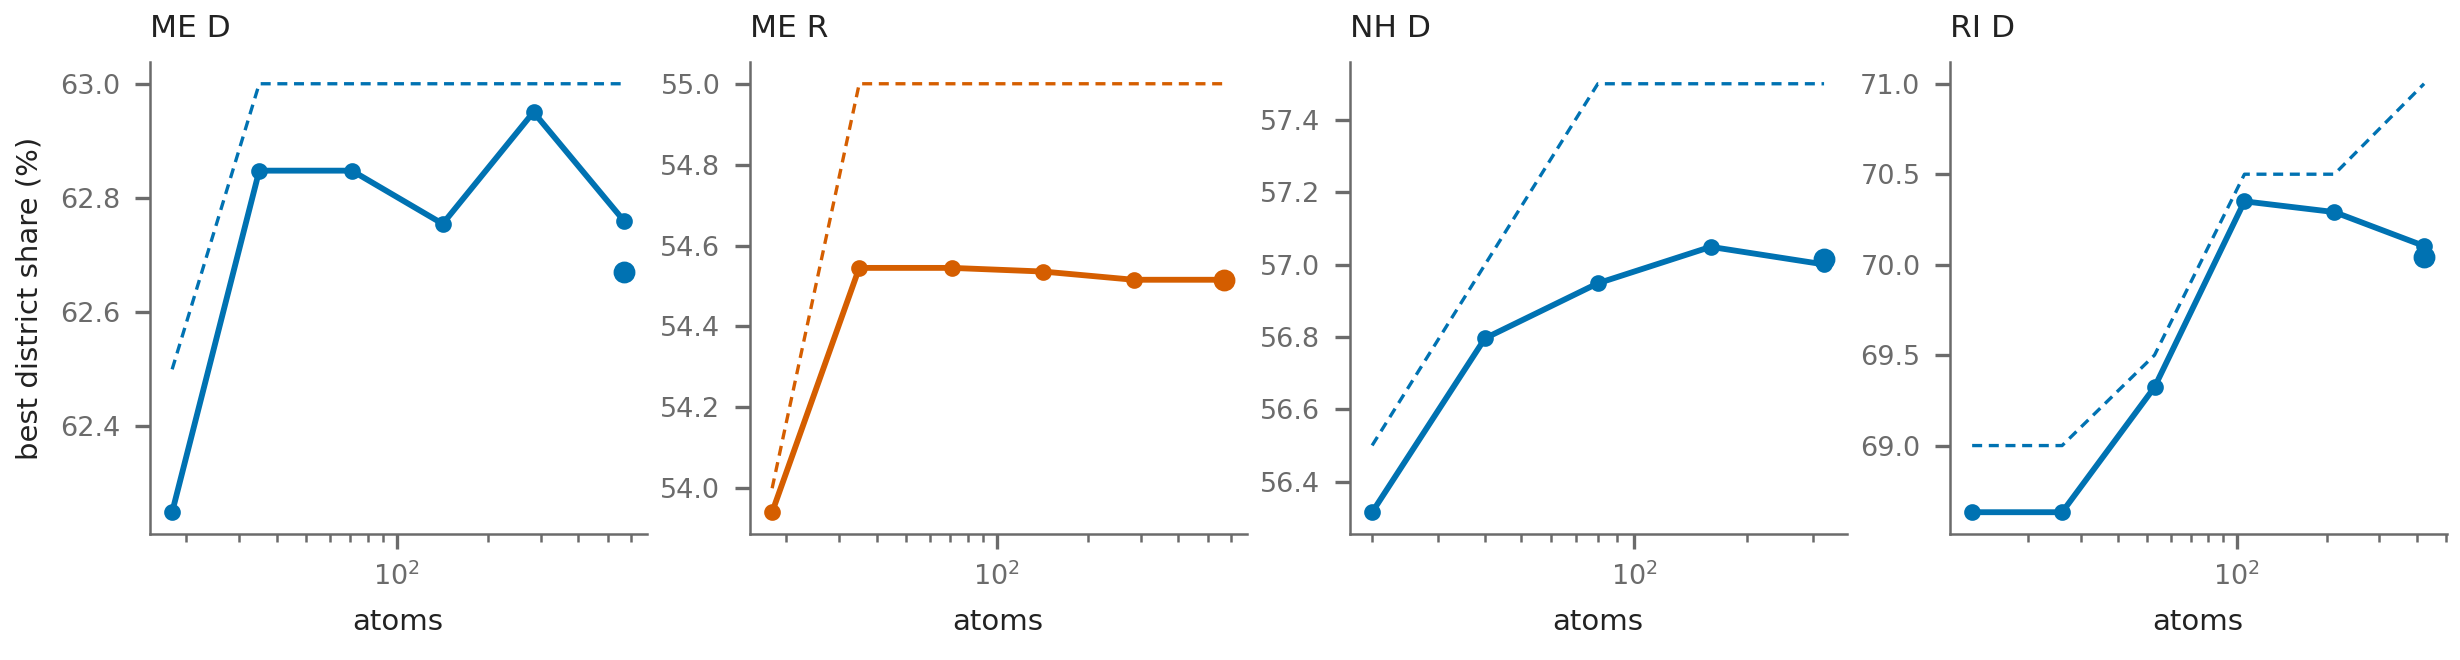
\includegraphics[width=\linewidth]{figs/ladder.png}
\caption{Resolution ladder: best-district share ($q=1$, $s=k-1$) when precincts are merged into fewer, larger atoms (plans keep merged atoms whole, so each rung is a lower-bound class for the next). Solid: best verified plan on the coarse instance; dashed: proven upper end for the coarse instance; large dot: the certified bracket at full precinct resolution. Non-monotone wiggles are heuristic search noise.}\label{fig:ladder}
\end{figure}

\paragraph{Resolution.}
Figure~\ref{fig:ladder} merges precincts, using the same homogeneity hierarchy as the algorithm, into $1/16,\dots,1/2$ as many atoms and recomputes the exact frontier. Because coarser atoms only shrink the plan class, each rung is a lower bound for the next, and the frontier saturates early: with a quarter of the precincts the best-district share is within 0.25 point of its precinct-level value in New Hampshire, Maine (both parties) and Rhode Island Democrats, and with a sixteenth it is within 0.7 point except in Rhode Island (1.5 points). This is evidence about sensitivity to \emph{coarser} atoms only; it does not bound what splitting precincts (or blocks, with an allocation model for the votes) could add.


\subsection{Audits and sanity checks}\label{sec:audit}

Every claim above is a lower bound (a plan) or an upper bound (an infeasibility proof), and each kind was checked separately.

\paragraph{Plans.}
All stored witness plans (514 plan records across the eight run sets) were re-verified from scratch after the runs by the independent verifier of Section~\ref{sec:data}, which recomputes labels, population, connectivity, split counts and every robust margin from raw data with rational arithmetic; none failed, and the exact $q$-th margin recomputed with fractions equals the recorded one. During the runs every plan returned by any solver was verified before it could enter a bracket; this caught one real bug (a cache keyed without the margin, which produced a plan that was not safe) that would otherwise have gone unnoticed.

\paragraph{Proofs.}
(i) \emph{Brute force.} On 72 random toy instances ($3\times4$ to $4\times5$ grids with random populations, votes and county labels, $k=2,3$, tolerance 20\%, budgets $s\in\{\infty,1,2\}$, both parties, several margins) the CEGAR answer for every $q$ equals the exact value from full enumeration of all plans, every relaxation along a random refinement chain is at least the exact value (validity), non-increasing along refinement (Theorem~\ref{thm:mono}), and equal to it at the atomic partition (Theorem~\ref{thm:exact}); none of the 72 failed. The pool relaxations, the safe-first decomposition and the county-aware recombination search pass 22 analogous checks. (ii) \emph{Second solver.} An independently written MILP encoding (single-commodity-flow connectivity, one linear split row, HiGHS with outer-safe tolerances) agrees with CP-SAT on 675 of 675 toy queries over all partitions of the refinement chains, on all 61 stored infeasibility proofs of the six two-district states (each re-derived by the loop and re-checked by HiGHS on the same final partition: 59 agree, 2 remain undecided after 300 s, none disagree), and on 163 of the 203 stored proofs of the states with three to five districts whose final partition is on file (the other 40 are undecided after 120 s; none disagree). An earlier random sample of 116 proofs gave the same picture (103 agree, 13 not re-derivable within the limit, 0 disagree). ``Undecided'' is never counted as agreement. The first version of this audit disagreed with CP-SAT on toy instances with $k=3$ and $s=2$ because the two encodings counted the budget differently (a bug in the audit encoding, not in the CEGAR model); after the fix all queries agree.

\paragraph{Sanity checks.}
(a) The statewide identity: no verified plan has $q=k$ safe districts above the statewide margin, and no proven upper end for $q=1$ lies below it. (b) Party symmetry: the pipeline run on New Hampshire with the two parties' votes exchanged returns the opposite party's brackets ($[57.02,57.5)$ and $[53.74,54.0)$ against $[57.02,57.5)$ and $[53.75,54.0)$). (c) Cross-run consistency: over 104 (state, party, $q$) keys with bounds from up to six independent run sets (and 248 keys across all regimes of Sections~\ref{sec:budget} and~\ref{sec:robust}), every verified lower end is strictly below every proven upper end. (d) Data: state populations equal the Census resident populations, statewide presidential totals reproduce the certified returns, atoms with more votes than residents hold under 0.7\% of the votes in every state. (e) Prior art: the geography-free hull bound, run on Massachusetts (nine districts; 2020 presidential vote, $\pm1\%$; not among our 16 states), allows Republicans at most one district with 50\% or more (best share below 52\%) and no second, in line with the finding of \citet{duchin2019} that Republicans are structurally locked out of district-sized collections of precincts there (their elections differ from ours, so the agreement is qualitative).

